% STATUS: ACTIVE -- three-page report extract (2026-08-06), for discussion.
%          p.1 figure  test_script/scratch/plot_formB_report_two_curves.m
%          p.2 figure  reused UNCHANGED from formB_selected_figs.tex p.8
%                      (figures/formB_bwide_seed{7,11}.png); caption condensed.
%          p.3 text    conclusion, stripped to the argument; every number that
%                      used to live here is in the two captions or in
%                      formB_selected_figs.tex pp.6-8.
% ======================================================
% Compile: xelatex formB_report_prior_belief.tex
% Path:    reference/eq17_analysis/derivation/formB_report_prior_belief.tex
% ======================================================

\documentclass[11pt,a4paper,fontset=none]{ctexart}

\usepackage[fleqn]{amsmath}
\usepackage{amssymb}
\setlength{\mathindent}{0pt}
\usepackage{geometry}
\geometry{margin=2.0cm}
\usepackage{graphicx}

\setlength{\parindent}{0pt}
\setlength{\parskip}{0.80em}
\linespread{1.08}

\begin{document}

\begin{center}
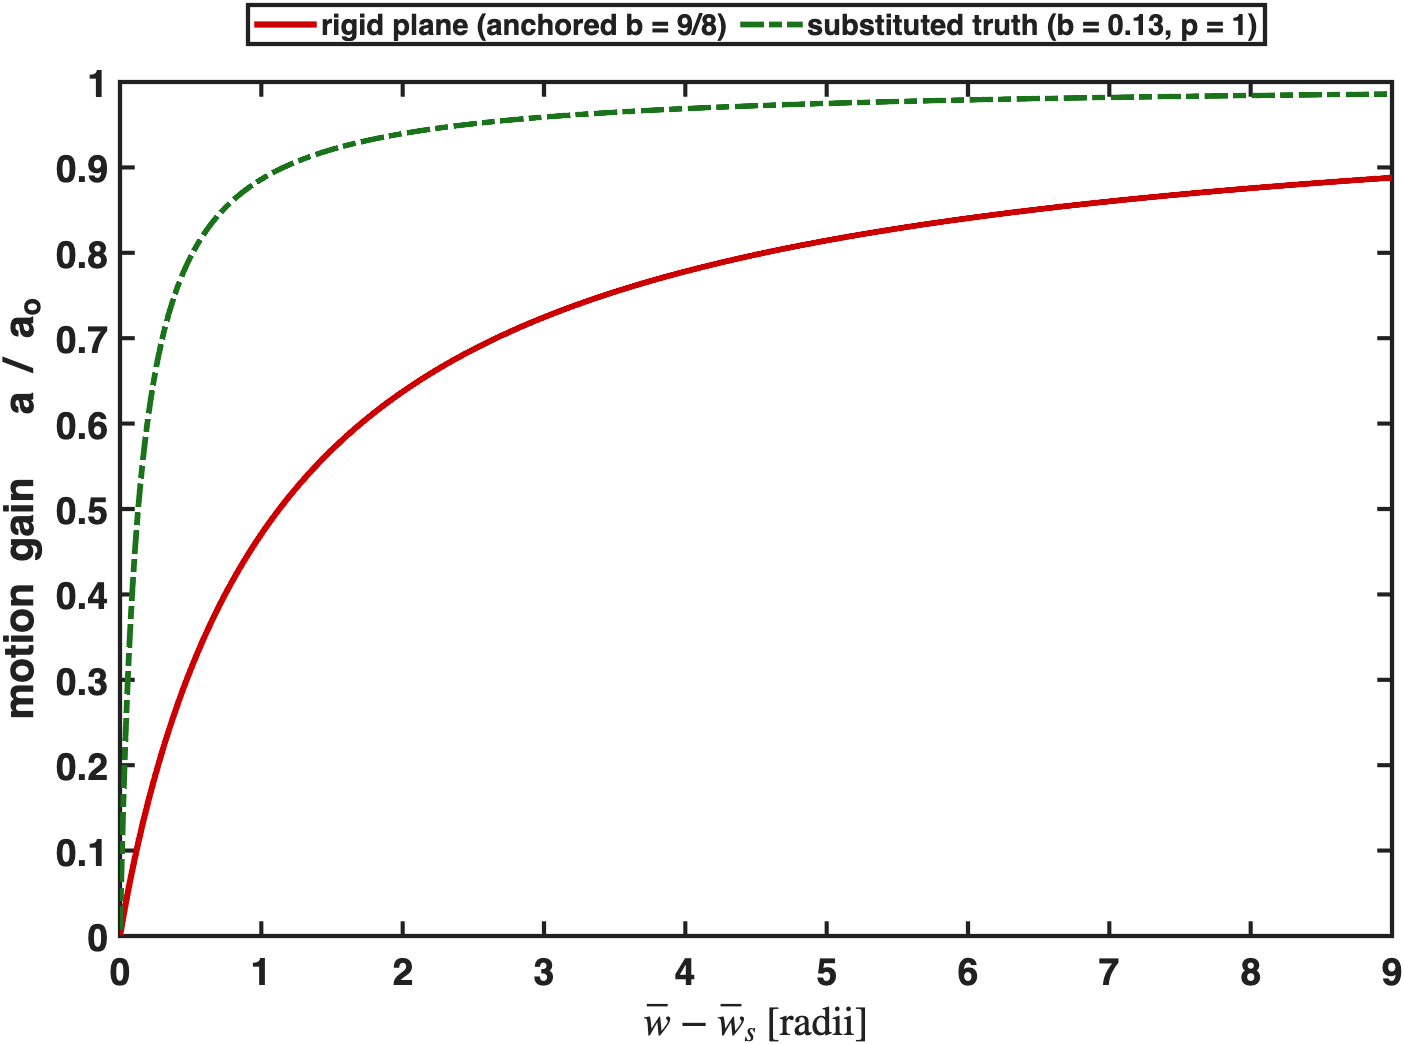
\includegraphics[width=0.78\linewidth]{figures/formB_report_two_curves.png}

The rigid plane our priors are anchored to (red), and the truth substituted on
the next page (dash-dot): same family, same contact point, $63.5$ prior widths
apart.
\end{center}

The controller does not estimate the gain height by height. It assumes the gain
follows one curve,
\[
\bar{a} \;=\; 1 - \left[\,\frac{b}{(\bar w - \bar w_s) + b}\,\right]^{p} ,
\]
and estimates only that curve's constants: $\bar w_s$, the contact position,
and $b$, the length over which the wall effect is spent. Whatever those
constants converge to, the gain is read off that shape and no other.

\clearpage

\begin{center}
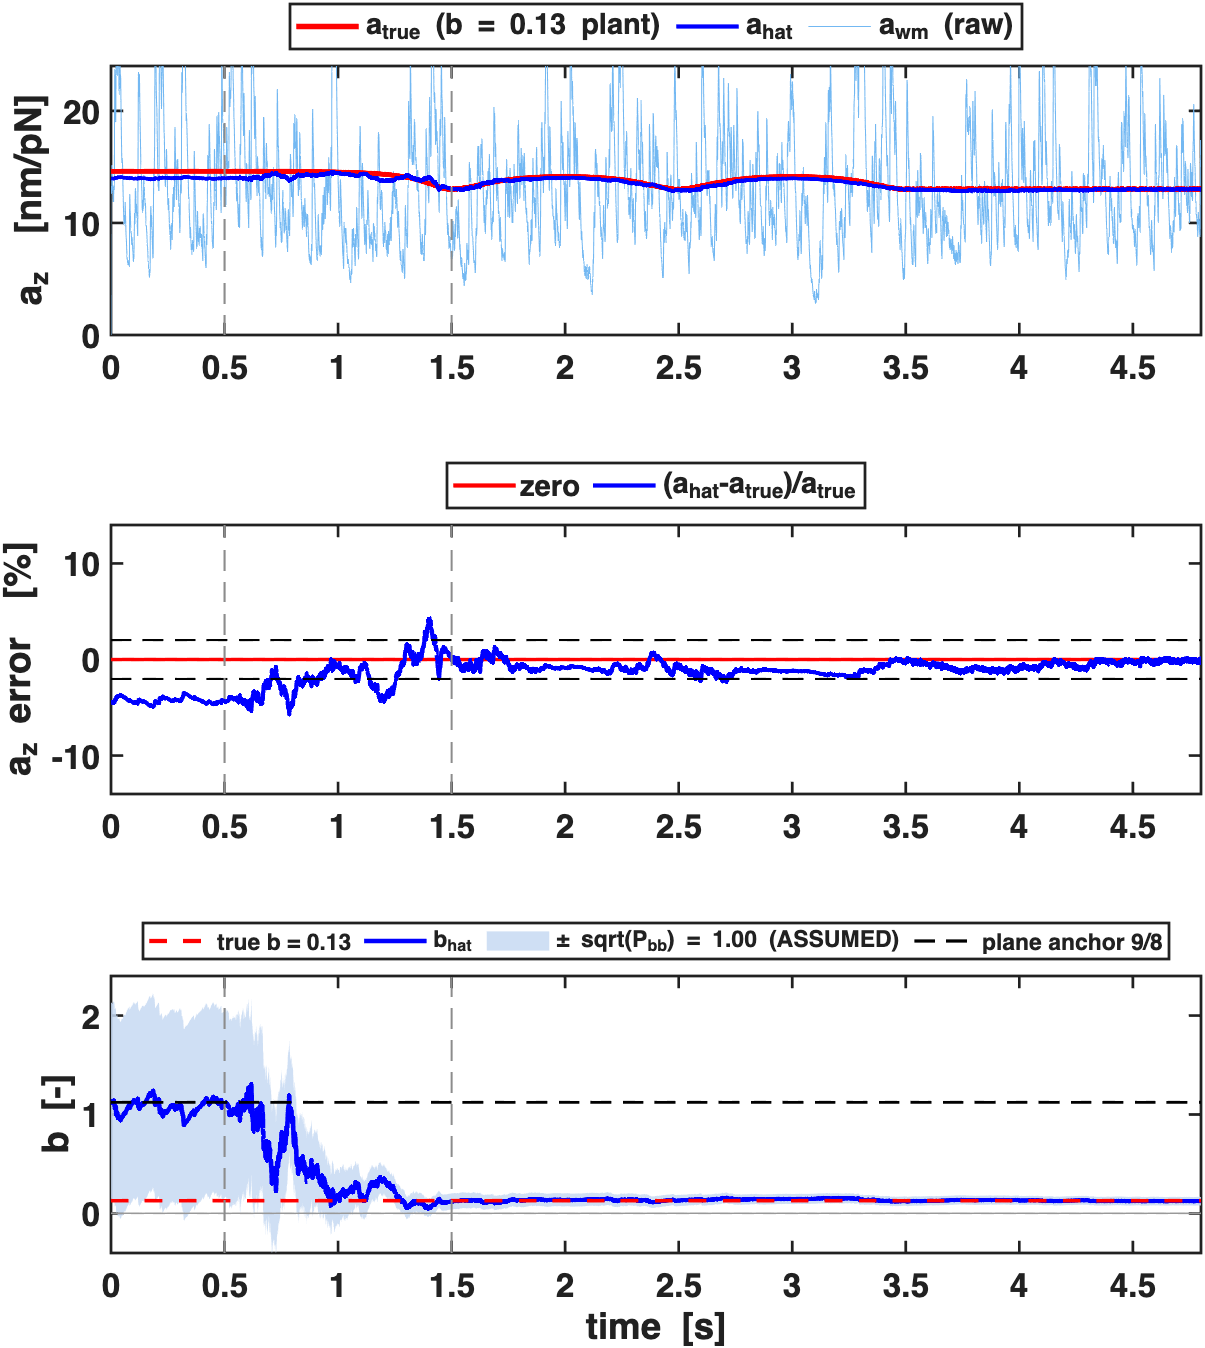
\includegraphics[width=0.49\linewidth]{figures/formB_bwide_seed7.png}\hfill
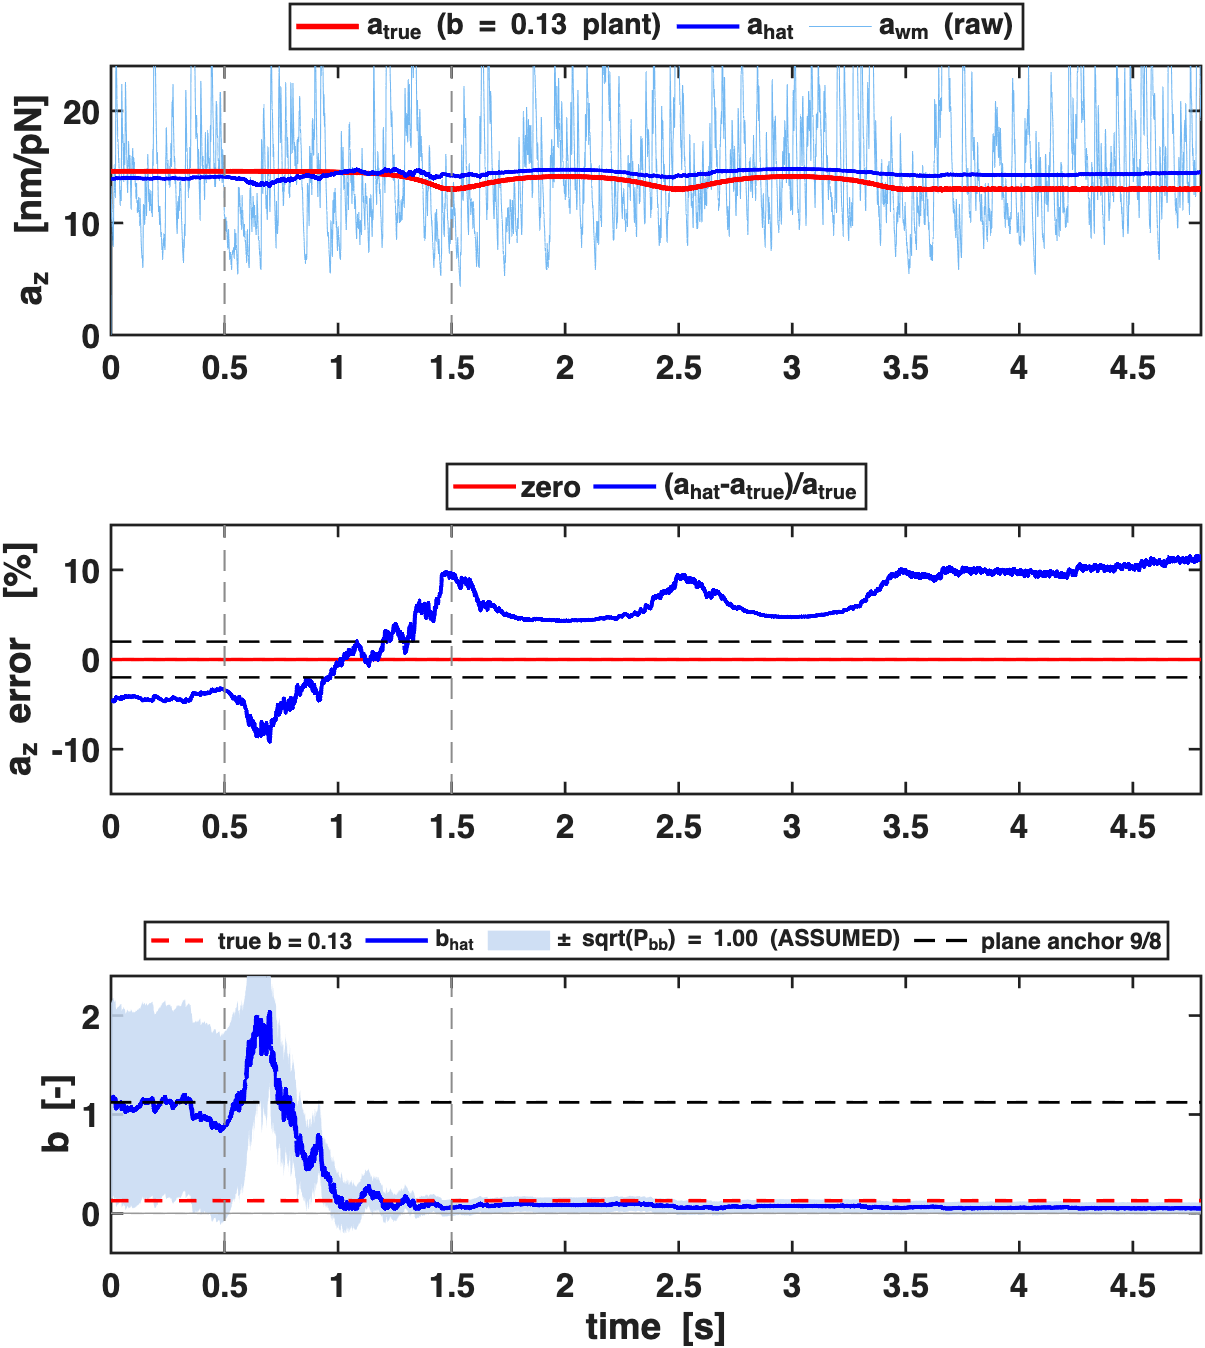
\includegraphics[width=0.49\linewidth]{figures/formB_bwide_seed11.png}

Widening the $b$ prior until the truth is inside it --- the widths are assumed,
not derived: the filter does reach the truth, but the answer becomes
seed-dependent.
\end{center}

\clearpage

$Q = 0$ is physically right --- $b$ is a constant, it does not drift. It also
means $P$ can only shrink: the filter gets one chance, and keeps whatever noise
that particular run happened to carry. Raising $Q$ is not the fix either. It
would claim $b$ drifts, which is false.

Neither choice is right, so what is missing is not a value of $Q$.

\begin{quote}
The model can say \emph{this constant does not change}.\\
It has no way to say \emph{my belief about it may be wrong}.\\
Both are carried by the same $Q$.
\end{quote}

The run itself already carries the evidence that the belief is wrong. There is
nowhere in the model to put it.

\end{document}
